% -----------------------------------------------------------------------------
%   Arquivo: ./01-texto/execucoes.tex
% -----------------------------------------------------------------------------

\section{Execuções}\label{sec:execucoes}    % edite para alterar o título da seção

Tendo-se implementado todas as classes, funções e estruturas necessárias para a simulação da rede social, executaram-se alguns testes para averiguar o correto funcionamento da busca em produndidade limitada.

A execução do programa é feita pelo seguinte comando:

{\tiny python -i profissionais.py}

Então, o python executa a geração da rede social e um terminal python é disponibilizado para a execução das simulações.

Todos os indivíduos encontram-se na lista indivíduos e para acessar um individuo, é necessário buscá-lo nessa lista. Se o indivíduo a ser acessado for o segundo, deve-se acessar a posição 1 da lista de indivíduos. Exemplo: individuos[1].

Tomando ainda como exemplo o segundo indivíduo, pela visualização gerada na biblioteca vis constata-se que esse indivíduo é um eletricista que é amigo dos individuos: 5 - gari, 12 - advogado e 14 - gari. Partindo-se deste indivíduo com o objetivo de encontrar um profissional que seja engenheiro, a execução da função profissionais deve retornar somente um profissional candidato: o indivíduo 19 - engenheiro que é amigo do individuo 12 - advogado, amigo do 1 - eletricista.

E a execução da função profissionais retornou exatamente só esse indivíduo candidato a dois níveis de distância, informando ainda o amigo que eles tem em comum - indivíduo 12, advogado.

Mais 10 execuções foram realizadas selecionando-se indivíduos aleatóriamente na rede social assim como suas profissões todos os resultados são validados na visualização da rede social.

A \textbf{Figura 7} mostra as execuções

\begin{figure*}
        \centering
        \caption{10 Execuções, validadas a olho nu com a visualização gráfica da rede social}
        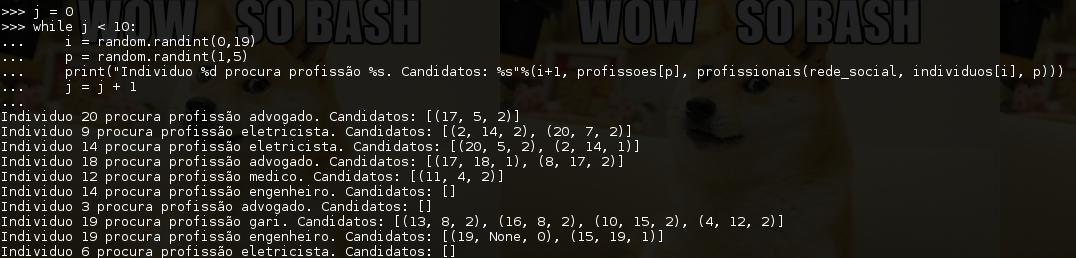
\includegraphics[scale=0.4]{./02-figuras/execucoes.png}
        \label{fig:execucoes}
\end{figure*}
